\section{Supply Chain Level Security Artifacts~\cite{slsa2023}}
A security framework provides checklist to ensure the integrity of the supply chain.
Artifacts that fulfill SLSA requirements endorsed a traceable source of the software provided
by trusted providers. SLSA provides trustworthiness of the artifacts to the developers, downstream users. 

\subsection{What is Software Supply Chain?}
Software supply chain is composed multiple components, first-party or third-
party libraries, and processes used to develop, build, test, and publish a software 
artifact \cite{DoDDefCI/CD2023}.

\subsection{Provenance}
SLSA provenance clearly provides the transparent information about the artifacts or the packages.
Information such as, who builds this artifact and how the artifact was built from the source.
These information will be verified by the package registory or even the customers. The provenance
is an attestion in SLSA.

\subsection{SLSA Provenance V.S SBOM (Software Bill of Materials)}
Provenance and SBOM are somehow similar, so they are easily confused. Provenance is used to 
assess the trustworthiness and security of the processes used to build and deliver the software artifacts~\ref{provenance}.
By contrast, SBOM focus on listing software components and their versions \ref{SBOM}.

\begin{lstlisting}[language=, caption=SLSA Provenance, label=provenance]
[Software Build Provenance]
Build Date: 2023-09-01
Build Environment: Secure, Isolated Environment
Signing Authority: Trusted Certificate Authority (CA)
Signature Verification: Passed
[Supply Chain Processes]
Code Review: Multi-stage code review by security experts
Dependency Scanning: Automated scanning for known vulnerabilities
Build Automation: Continuous Integration/Continuous Deployment (CI/CD) pipeline
Deployment: Automated deployment to secure servers
[Organizations Involved]
Development Team: Responsible for code development
Security Team: Responsible for security reviews and scanning
Operations Team: Responsible for deployment
\end{lstlisting}

\begin{lstlisting}[language=, caption=SBOM, label=SBOM]
[MyApp (v1.0)]
Frontend Framework (v2.3)
Database Connector (v1.1)
Authentication Library (v3.0)
Logging Utility (v1.2)
\end{lstlisting}

\subsection{Build Model}
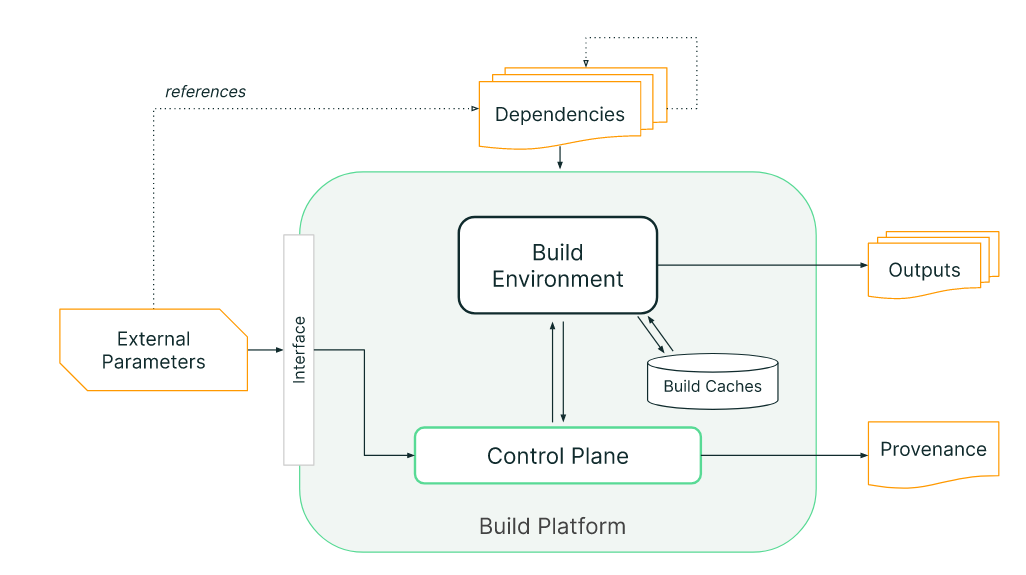
\includegraphics[width=0.7\textwidth]{./screenshot/build_model.png}
\begin{enumerate}
  \item The tenant (developers) provide specific external parameters, like the version of the application 
  and the reference to the dependency.
  \item The control plane receives the external parameters, then fetch the necessary build scripts, configuration,  
  and depencies based on the external parameters.
  \item The control system sets up the isolated environment for the build.
  \item Finally, the model outputs the artifacts. If the build platform follows SLSA build level 2+, then
  the provenance will also be generated from the control systems.
\end{enumerate}
\subsection{SLSA Security Level}
Currently SLSA have defined 4 levels (LV.0 - LV.3), which will be 
briefly described in Table~\ref{tab:slsa-levels}, and working on level 4.
\begin{table}[ht]
  \centering
  \caption{SLSA Security Levels}
  \label{tab:slsa-levels}
  \begin{tabular}{|c|c|p{6cm}|}
  \hline
  \textbf{Level} & \textbf{Requirements} & \textbf{Focus} \\
  \hline
  Build L0 & None & No security practices are in place. \\
  \hline
  Build L1 & With provenance & Basic security practices are followed, such as code review and basic dependency scanning. \\
  \hline
  Build L2 & Signed provenance, generated by a hosted build platform & More comprehensive security practices are implemented, including in-depth code review, vulnerability scanning, and build verification. \\
  \hline
  Build L3 & Hardened build platform & The highest level of security is maintained, with strict adherence to security practices, automated testing, and supply chain integrity checks. \\
  \hline
  \end{tabular}
\end{table}


